\documentclass[conference]{IEEEtran}
\IEEEoverridecommandlockouts
% The preceding line is only needed to identify funding in the first footnote. If that is unneeded, please comment it out.
\usepackage{cite}
\usepackage{amsmath,amssymb,amsfonts}
\usepackage{algorithmic}
\usepackage{graphicx}
\usepackage{textcomp}
\usepackage{float}


\usepackage{xcolor}
%\usepackage[svgnames]{xcolor}
%\usepackage[capposition=bottom]{floatrow}
\usepackage{listings}
\usepackage{footnote}
\definecolor{dkgreen}{rgb}{0,0.6,0}
\definecolor{gray}{rgb}{0.5,0.5,0.5}
\definecolor{mauve}{rgb}{0.58,0,0.82}
\lstset{
  basicstyle=\ttfamily,
  columns=fullflexible,
  frame=single,
  breaklines=true,
  postbreak=\mbox{\textcolor{red}{$\hookrightarrow$}\space},
}
\lstset{ %
  language=R,                     % the language of the code
  basicstyle=\footnotesize,       % the size of the fonts that are used for the code
  numbers=left,                   % where to put the line-numbers
  numberstyle=\tiny\color{gray},  % the style that is used for the line-numbers
  stepnumber=1,                   % the step between two line-numbers. If it's 1, each line
                                  % will be numbered
  numbersep=5pt,                  % how far the line-numbers are from the code
  backgroundcolor=\color{white},  % choose the background color. You must add \usepackage{color}
  showspaces=false,               % show spaces adding particular underscores
  showstringspaces=false,         % underline spaces within strings
  showtabs=false,                 % show tabs within strings adding particular underscores
  frame=single,                   % adds a frame around the code
  linewidth=0.47\textwidth,
  rulecolor=\color{black},        % if not set, the frame-color may be changed on line-breaks within not-black text (e.g. commens (green here))
  tabsize=2,                      % sets default tabsize to 2 spaces
  captionpos=b,                   % sets the caption-position to bottom
  breaklines=true,                % sets automatic line breaking
  breakatwhitespace=false,        % sets if automatic breaks should only happen at whitespace
  title=\lstname,                 % show the filename of files included with \lstinputlisting;
                                  % also try caption instead of title
  keywordstyle=\color{blue},      % keyword style
  commentstyle=\color{dkgreen},   % comment style
  stringstyle=\color{mauve},      % string literal style
  escapeinside={\%*}{*)},         % if you want to add a comment within your code
  morekeywords={*,...}            % if you want to add more keywords to the set
} 


\def\BibTeX{{\rm B\kern-.05em{\sc i\kern-.025em b}\kern-.08em
    T\kern-.1667em\lower.7ex\hbox{E}\kern-.125emX}}
\begin{document}

\title{Music Trending Analysis Based on Spotify Data\\
%{\footnotesize \textsuperscript{*}Note: Sub-titles are not captured in Xplore and
%should not be used}
\thanks{University of Central Florida}
}

\author{\IEEEauthorblockN{1\textsuperscript{st} Trent Zhang}
\IEEEauthorblockA{\textit{dept. Statistics} \\
\textit{University of Illinois at Urbana-Champaign}\\
Urbana, IL \\
zz90@illinois.edu}
}

\maketitle

\begin{abstract}
First, we tried few statistical model to know what are the largest influencers on a song’s success based on the features extracted from spotify. For top 20 \% popular musics, our regression model gives reasonable out-of-sample predictions: ±4.86 based on root-mean-squared-error.
Then, we tried multinomial logistic regression, linear discriminative analysis, quadratic discriminative analysis, k-nearest neighbors and decision tree to classify whither a song is popular or not. The best classification model is KNN (K=2) gives out-of-sample predictive over all error rate: 0.391 based on 0-1-error, and error rate of 0.3953 on popular songs.
\end{abstract}

\begin{IEEEkeywords}
Trend Prediction, Music Analysis, Regression Analysis
\end{IEEEkeywords}

\section{Introduction}
\subsection{Background}
In 2017, the music industry generated \$8.72 billion in the United States alone. Thanks to growing streaming services (Spotify, Apple Music, etc) the industry continues to flourish. Popular songs secure the lion’s share of revenue. The top 10 artists in 2016 generated a combined \$362.5 million in revenue. The question of what makes a song popular has been studied before with varying degrees of success. Every song has key characteristics including lyrics, duration, artist information, temp, beat, loudness, chord, etc.

\subsection{Problem Description}
 We decided to further investigate by asking three key questions: 
\begin{enumerate}
  \item Are there certain characteristics for hit songs?
  \item What are the largest influencers on a song’s success?
  \item Can we predict the popularity of new songs? 
\end{enumerate}

\section{Data Preparation}
\subsection{Data Source}
Predicting how popular one track will be a hard task. To answer these questions, we made use of Spotify Audio Features (Audio features for 115k tracks collected from the official Spotify Web API) provided by tomigelo from kaggle\cite{tomigelo_2018}, which covered the tracks that released between January 2018 to April 2019.

\subsection{Data Content}
This dataset has altogether 130633 row and 17 column. Each track (row) has values for artist name, track name, track id and the audio features\cite{spotifyfordevelopers} itself. Additionally, there is also a popularity feature which is changing over time so it might not be up-to-date when we access the data. All features are listed as TABLE \ref{Features of original data}

% latex table generated in R 3.5.2 by xtable 1.8-4 package
% Thu Dec  5 03:25:13 2019
\begin{table}[ht]
\centering
\caption{Features of original data}
\label{Features of original data}
\begin{tabular}{rlll}
  \hline
 & Features & &Features\\ 
  \hline
1 & artist\_name & 11 & loudness \\ 
  2 & track\_id &12 & mode\\ 
  3 & track\_name &13 & speechiness\\ 
  4 & acousticness &14 & tempo \\ 
  5 & danceability &15 & time\_signature \\ 
  6 & duration\_ms &16 & valence\\ 
  7 & energy &17 & popularity \\ 
  8 & instrumentalness &\\ 
  9 & key &\\ 
  10 & liveness &\\ 
   \hline
\end{tabular}
\end{table}

\subsection{Data Split}
The total data is randomly split into train data (70\%) and validation data (30\%).

\section{Descriptive Analysis} 
We depict scatter, density and correlation plot of our numeric variables as Fig. \ref{ggpairs.pdf}, and have some insights from it as follows:
\begin{itemize}
  \item The more energy, the more loudness;
  \item Most of popular tracks are loud;
  \item Most of tracks are non-live, loud, non-speech, 4/4 time signature;
  \item The popularity data is significantly right skewed.
\end{itemize}


\begin{figure}[htbp]
\centerline{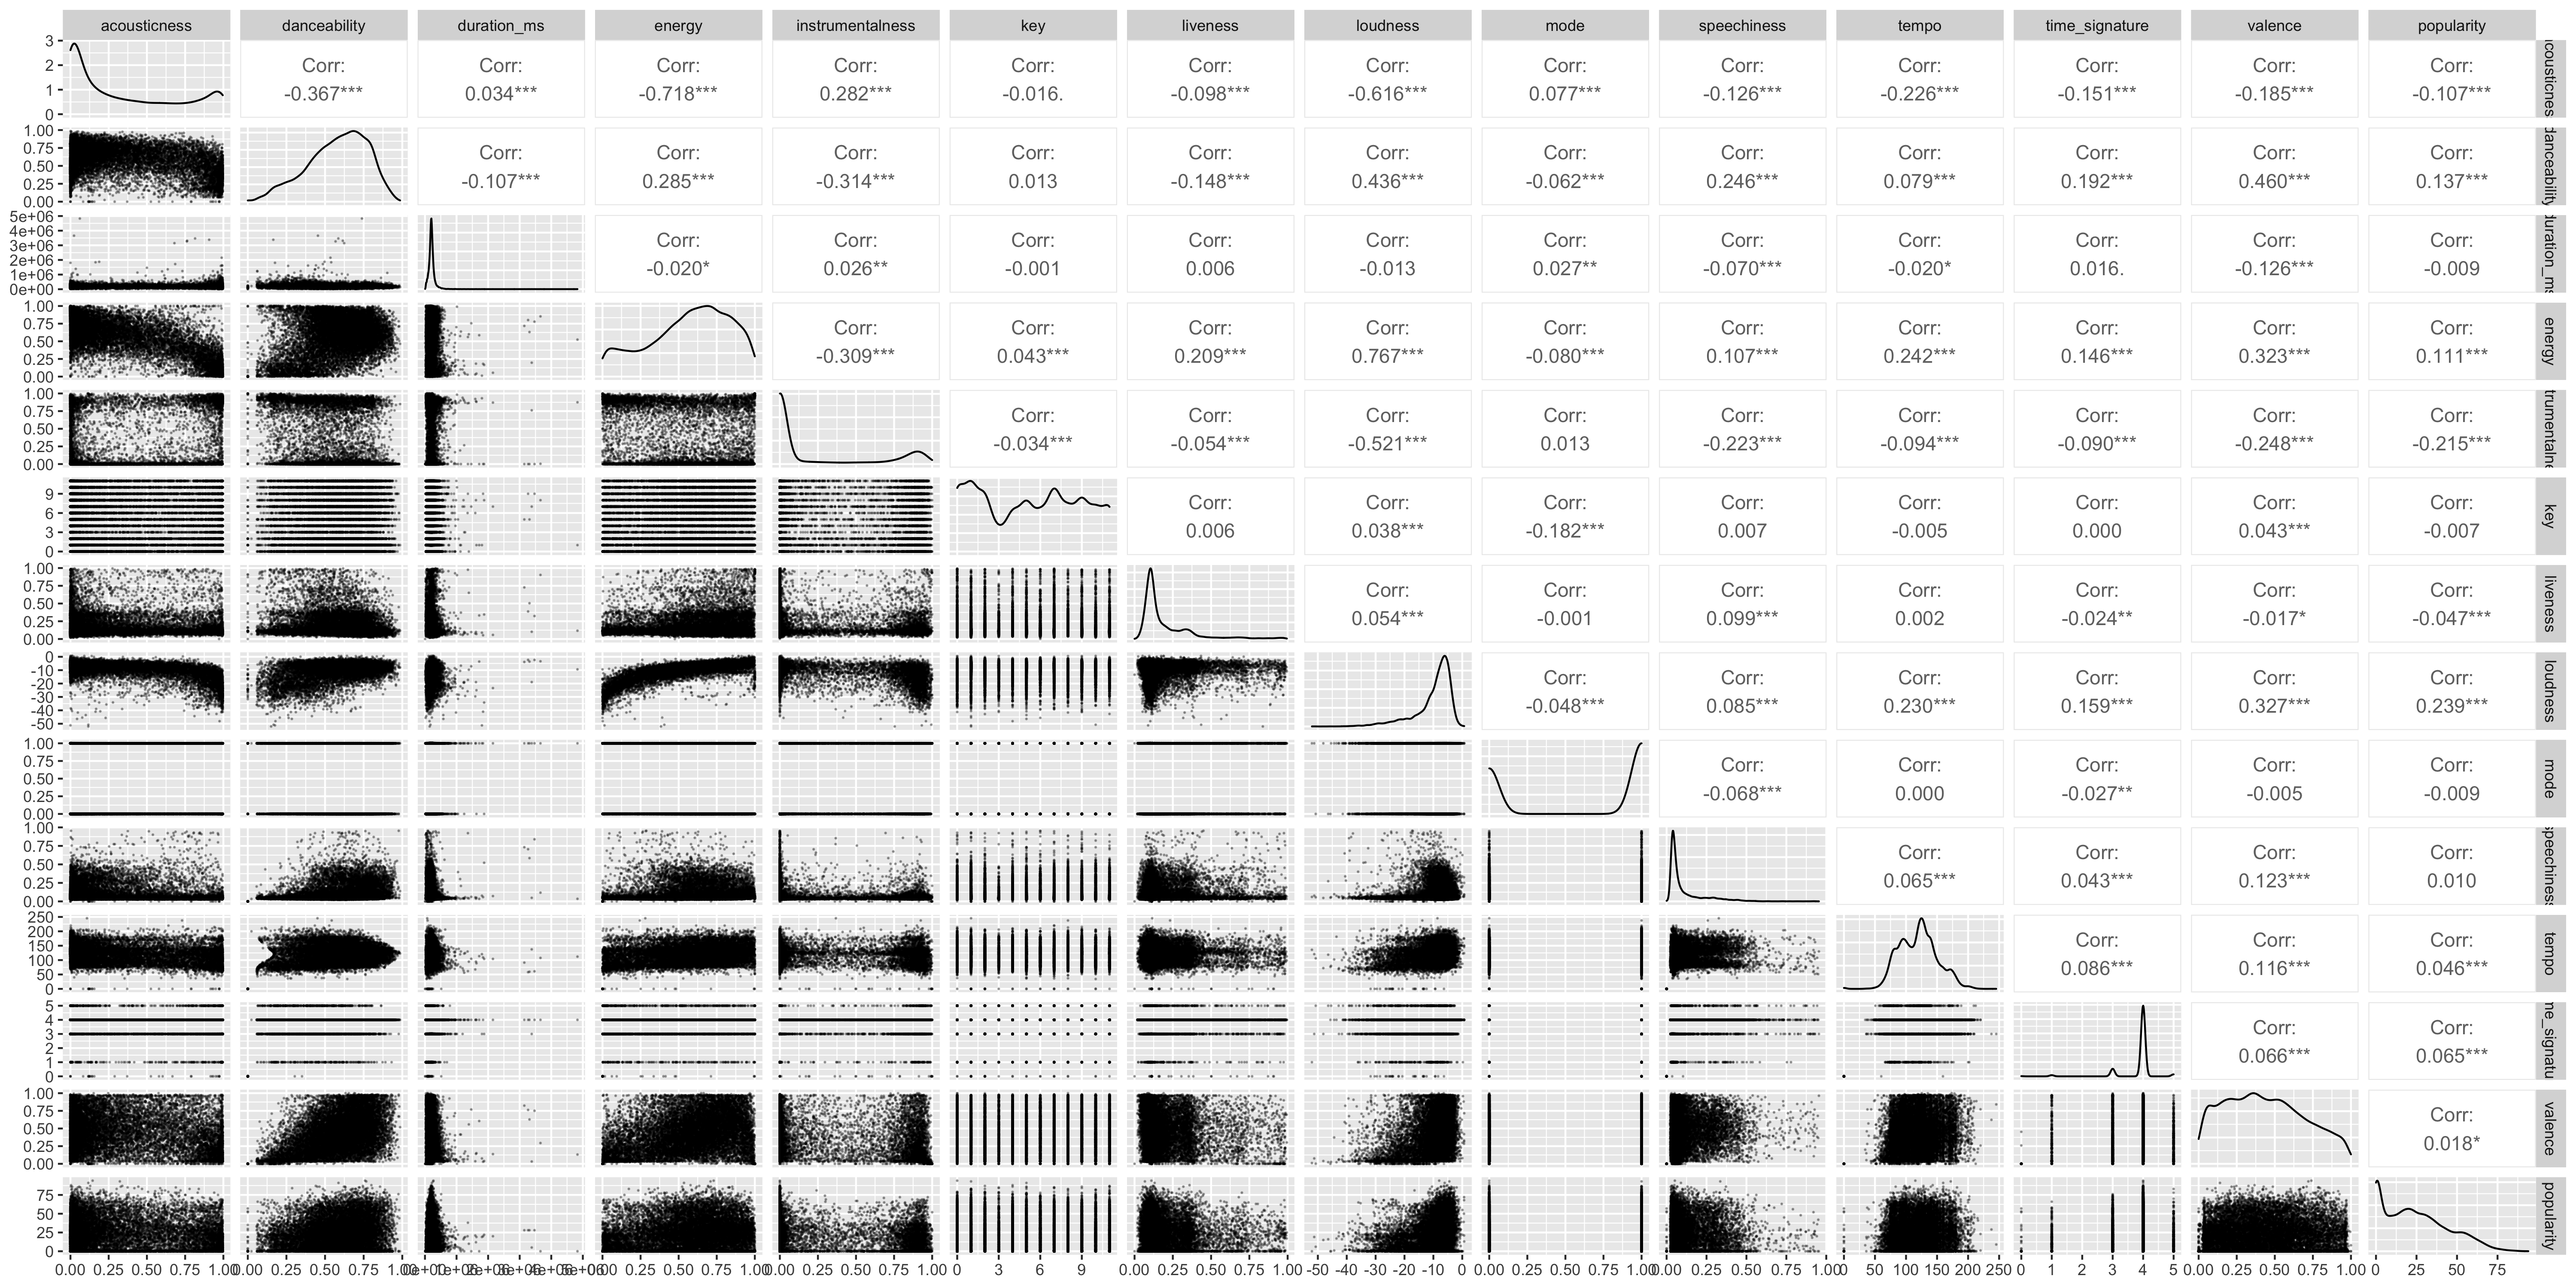
\includegraphics[width=0.49\textwidth]{figure/ggpairs.png}}
\caption{Scatter, density and correlation plots}
\label{ggpairs.pdf}
\end{figure}

\section{Regressive Model Analysis of Top 20\% Popular Song}
In this section, in order to know what are the largest influencers on a song’s success. We discuss the results of the multiple regression model, ridge model, Lasso model and elastic-net model based on Top 20\% Popular Song. Cross validation is used to evaluate the result of model.


\subsection{The Multiple Regression Model}\label{The Multiple Regression Model}
We use linear regression with all variable and get a model with RMSE as TABLE \ref{RMSE Table of Linear regression}. Fig. \ref{Prediction Versus The Observation in train} shows the prediction versus the observation when we use all train data to fit the model. Fig. \ref{Prediction Versus The Observation in test} shows the prediction versus the observation when we use the model to test data. 

From the figure, test error and we can know that Linear regression is not good at predicting popularity of one track. 

\begin{table}[ht]
\centering
\caption{Coefficient of Linear regression}
\begin{tabular}{rr}
  \hline
 & coefficients \\ 
  \hline
(Intercept) & 85.10 \\ 
  acousticness & -0.14 \\ 
  danceability & 4.26 \\ 
  duration\_ms & -0.00 \\ 
  energy & -2.05 \\ 
  instrumentalness & -1.26 \\ 
  key & -0.07 \\ 
  liveness & 1.50 \\ 
  loudness & 0.01 \\ 
  mode & 0.10 \\ 
  speechiness & 0.78 \\ 
  tempo & -0.02 \\ 
  time\_signature & 0.53 \\ 
  valence & -0.00 \\ 
   \hline
\end{tabular}
\label{Coefficient of Linear regression}		
\end{table}

\begin{figure}[htbp]
\centerline{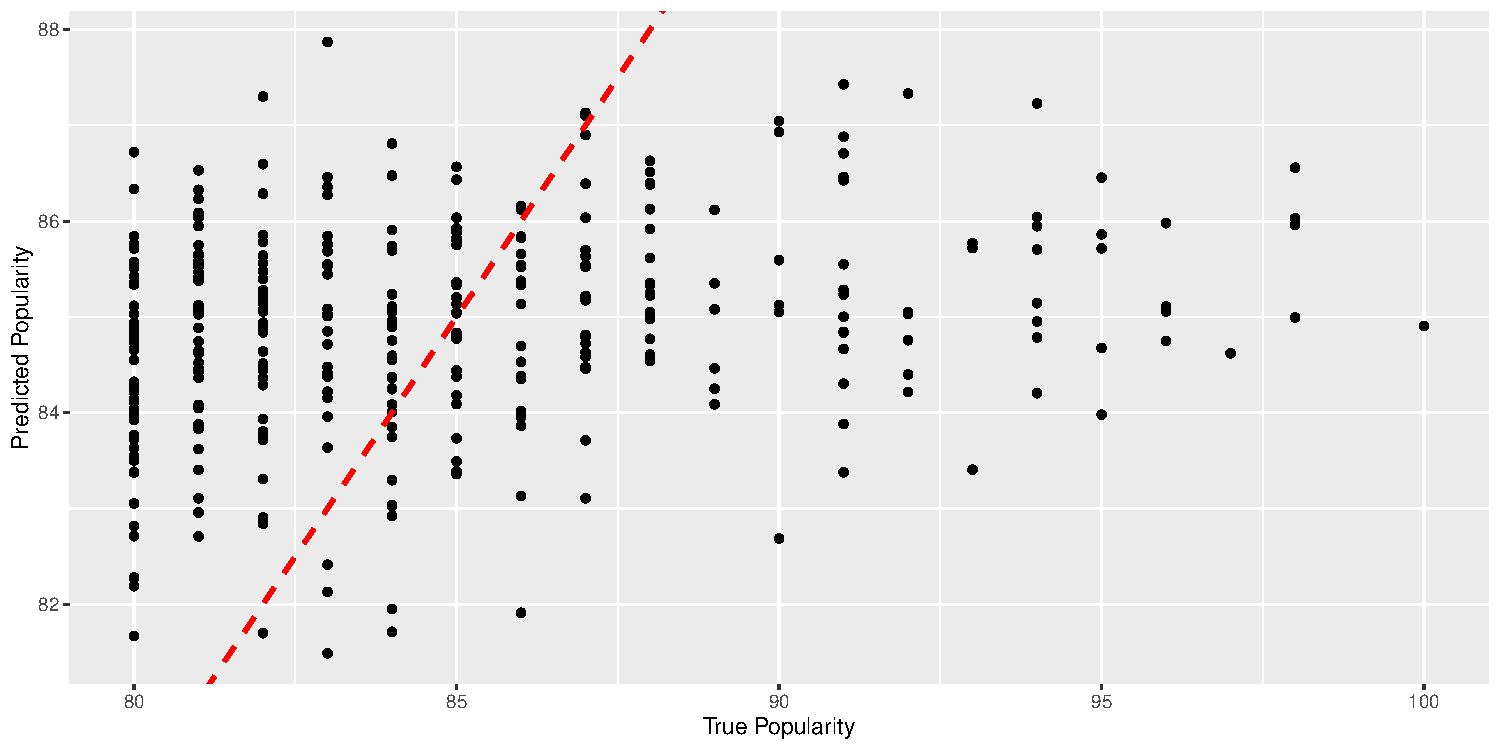
\includegraphics[width=0.5\textwidth]{figure/predict_and_observe_plot.pdf}}
\caption{Prediction Versus The Observation in train}
\label{Prediction Versus The Observation in train}
\end{figure}


\begin{figure}[htbp]
\centerline{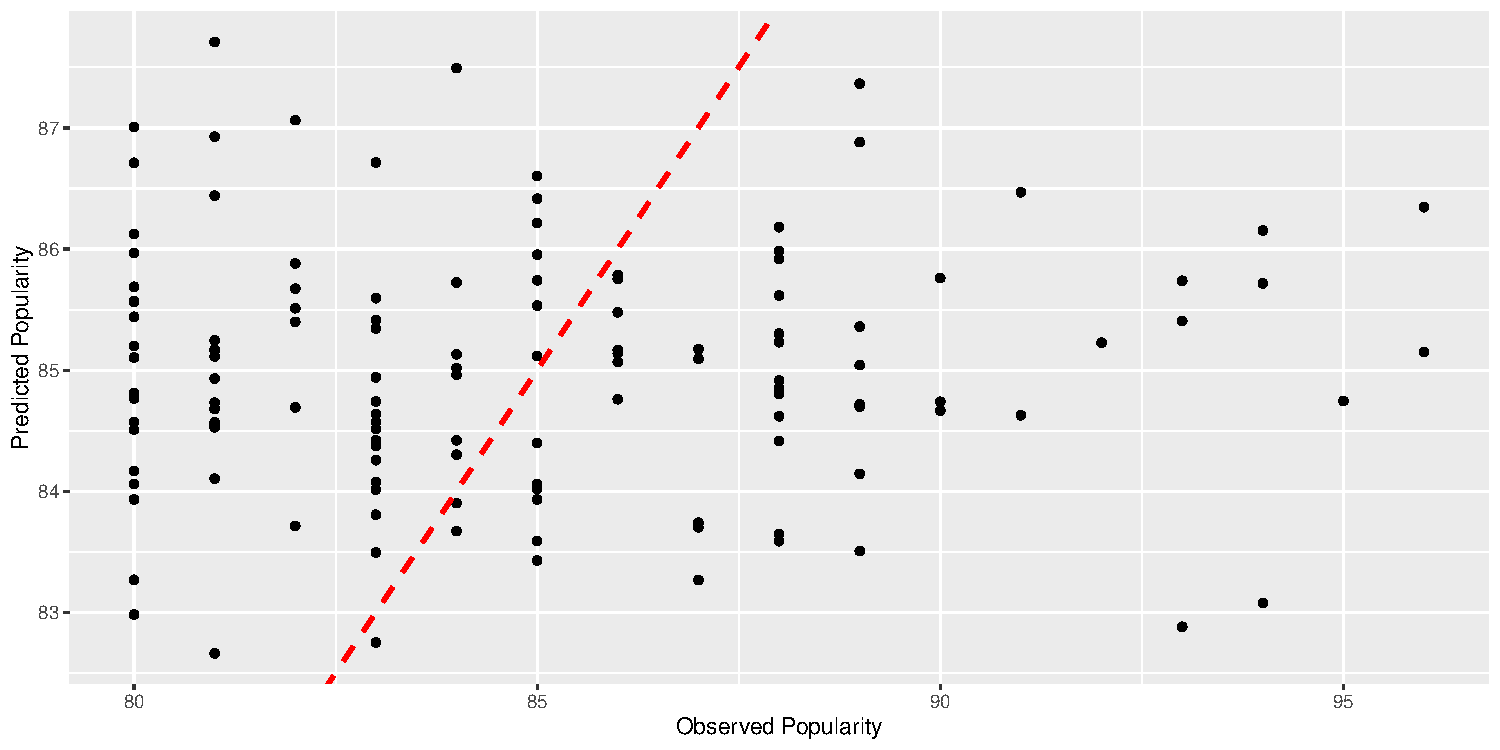
\includegraphics[width=0.5\textwidth]{figure/testerror.pdf}}
\caption{Prediction Versus The Observation in test}
\label{Prediction Versus The Observation in test}
\end{figure}


\begin{table}[ht]
\centering
\caption{RMSE Table of Linear regression}
\begin{tabular}{rr}
  \hline
rmse.lm.train & rmse.lm.test \\ 
  \hline
4.04 & 4.86 \\ 
   \hline
\end{tabular}
\label{RMSE Table of Linear regression}	
\end{table}
	


\subsection{Ridge with Cross Validation}
But we noticed that there are many variables in this model and the some of the variable is statistically insignificant. Therefore, variable selection is needed. 

We first use Ridge regression. The result is shown as Fig. \ref{Total Number of Coefficient and RMSE in Ridge}. From the result, we can see that the error bar range is Large and the minimum RMSE is at $\log\lambda=-1.65$. Obviously, the ridge regression makes substantial improvements in improving test RMSE compared to the linear regression model which mainly because of the penalty.

\begin{figure}[htbp]
\centerline{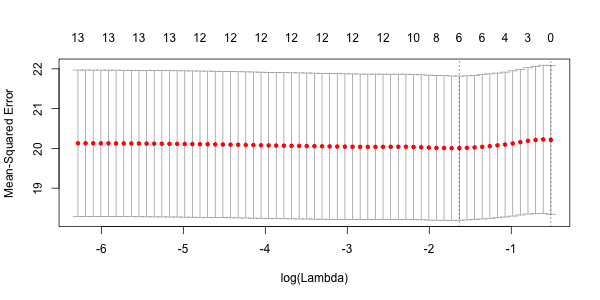
\includegraphics[width=0.5\textwidth]{figure/cvfitlasso.png}}
\caption{Total Number of Coefficient and RMSE in Ridge\protect\footnotemark}
\label{Total Number of Coefficient and RMSE in Ridge}
\end{figure}
\footnotetext{Red point is the mean RMSE of 10 Cross Validations, gery error bar is the uppermost and lowermost RMSE of 10 fold Cross Validation, the two dashed lines are value of lambda that gives minimum RMSE and largest value of lambda such that error is within 1 standard error of the minimum. The following similar figures' elements are the same as this figure.}

\begin{table}[ht]
\centering
\caption{Coefficient of Ridge regression}
\begin{tabular}{rr}
  \hline
 & s0 \\ 
  \hline
acousticness & -0.06 \\ 
  danceability & 1.86 \\ 
  duration\_ms & -0.00 \\ 
  energy & -0.73 \\ 
  instrumentalness & -0.87 \\ 
  key & -0.02 \\ 
  liveness & 0.54 \\ 
  loudness & -0.03 \\ 
  mode & -0.01 \\ 
  speechiness & 0.35 \\ 
  tempo & -0.01 \\ 
  time\_signature & 0.27 \\ 
  valence & 0.10 \\ 
   \hline
\end{tabular}
\label{Coefficient of Ridge regression}		
\end{table}

\subsection{LASSO with Cross Validation}
LASSO is a regression analysis method which performs both variable selection and regularization in order to improve prediction accuracy and interpretability of the statistical model it produces\cite{tibshirani1996regression}. By LASSO we can greatly shrink the number of variable and balance the accuracy of the model.However, there is a parameter $\lambda$ needed to tune, in order to make the objectivity of choosing $\lambda$, here we use 10th Cross Validation\cite{kohavi1995study}. 

The result is shown as Fig. \ref{Total Number of Coefficient and RMSE in Lasso}. From the result, we can see that the error bar range is Large and the minimum RMSE is at $\log\lambda=-1.65$. Obviously, the LASSO makes substantial improvements in improving test RMSE compared to the linear regression model which mainly because of the penalty. Besides, LASSO can also make some coefficient to $0$. From the coefficient TABLE \ref{Coefficient of LASSO regression} we can see the following imformation:
\begin{enumerate}
  \item The higher danceability, the higher popularity;
  \item The lower energy, the higher popularity.
\end{enumerate}
 

\begin{figure}[htbp]
\centerline{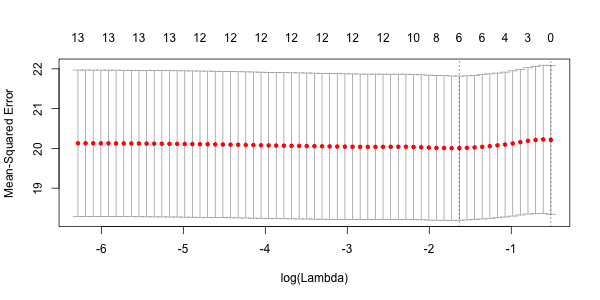
\includegraphics[width=0.5\textwidth]{figure/cvfitlasso.png}}
\caption{Total Number of Coefficient and RMSE in Lasso}
\label{Total Number of Coefficient and RMSE in Lasso}
\end{figure}

\begin{table}[ht]
\centering
\caption{Coefficient of LASSO regression}
\begin{tabular}{rr}
  \hline
 & s0 \\ 
  \hline
acousticness & 0.00 \\ 
  danceability & 2.90 \\ 
  duration\_ms & -0.00 \\ 
  energy & -0.58 \\ 
  instrumentalness & 0.00 \\ 
  key & -0.00 \\ 
  liveness & 0.00 \\ 
  loudness & 0.00 \\ 
  mode & 0.00 \\ 
  speechiness & 0.00 \\ 
  tempo & -0.02 \\ 
  time\_signature & 0.00 \\ 
  valence & 0.00 \\ 
   \hline
\end{tabular}
\label{Coefficient of LASSO regression}		
\end{table}

\subsection{Elastic-net with Cross Validation}
Elastic Net first emerged as a result of critique on lasso, whose variable selection can be too dependent on data and thus unstable. The solution is to combine the penalties of ridge regression and lasso to get the best of both worlds. Elastic Net aims at minimizing the following loss function:

\begin{equation}
  \frac{\sum\limits_{i-1}^{n}\left(y_{i}-x_{i}^{\prime} \hat{\beta}\right)^{2}}{2 n}+\lambda\left(\frac{1-\alpha}{2} \sum_{j=1}^{m} \hat{\beta}_{j}^{2}+\alpha \sum_{j=1}^{m}\left|\hat{\beta}_{j}\right|\right)
\end{equation}
where $\alpha$ is the mixing parameter between ridge ($\alpha=0$) and lasso ($\alpha=1$).

The result is shown as Fig. \ref{Total Number of Coefficient and RMSE in Elastic-net}. From the result, we can see that the best Elastic-net is similar to LASSO model.

\begin{figure}[htbp]
\centerline{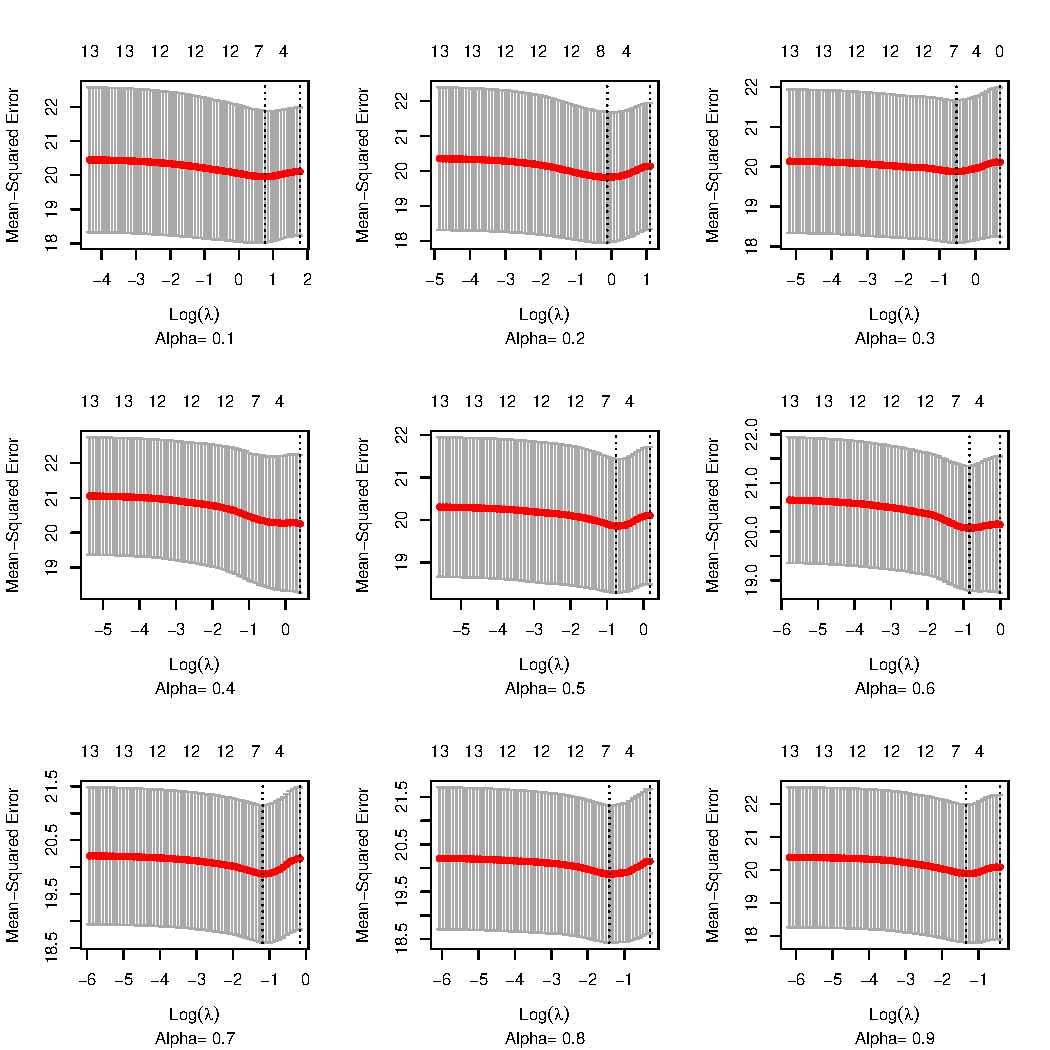
\includegraphics[width=0.5\textwidth]{figure/cvfitpla_net.pdf}}
\caption{Total Number of Coefficient and RMSE in Elastic-net}
\label{Total Number of Coefficient and RMSE in Elastic-net}
\end{figure}

\begin{table}[ht]
\centering
\caption{Coefficient of Elastic-net regression}
\begin{tabular}{rr}
  \hline
 & Coefficient \\ 
  \hline
acousticness & 0.00 \\ 
  danceability & 2.34 \\ 
  duration\_ms & -0.00 \\ 
  energy & -0.25 \\ 
  instrumentalness & 0.00 \\ 
  key & 0.00 \\ 
  liveness & 0.00 \\ 
  loudness & 0.00 \\ 
  mode & 0.00 \\ 
  speechiness & 0.00 \\ 
  tempo & -0.01 \\ 
  time\_signature & 0.00 \\ 
  valence & 0.00 \\ 
   \hline
\end{tabular}
\label{Coefficient of Elastic-net regression}		
\end{table}





\section{Classificative Model Analysis}
In this chapter, we use multinomial logistic regression, linear discriminative analysis, quadratic discriminative analysis, tree method, random forest and k-nearest neighbors\cite{james2013introduction} to classify our data. All model result is trained by 10-fold cross validation within the train data. Before classification, we divide the popularity data to 3 classes as TABLE \ref{Divid the data to 3 classes}.

\begin{table}[ht]
\centering
\caption{Divid the data to 3 classes}
\begin{tabular}{rrrr}
  \hline
&Unpopular & Normal & Popular \\ 
  \hline
Popularity& 0-40& 40-70&70-100 \\ 
Train Count&26621 & 63406 &1437 \\                                           
   \hline
\end{tabular}
\label{Divid the data to 3 classes}		
\end{table}
In this table, we noticed that our data is highly imbalanced, if we use this data directly, our classification model might be highly biased towards the category which has the highest samples. Hence, we balanced the data, the way we use to balance the data subsample. 
\begin{table}[ht]
  \centering
  \caption{Balanced Data}
  \begin{tabular}{rrrr}
    \hline
  &Unpopular & Normal & Popular \\ 
    \hline
  Popularity& 0-40& 40-70&70-100 \\ 
  Train Count&1437 & 1437 &1437 \\                                           
     \hline
  \end{tabular}
  \label{Balanced Data}		
  \end{table}

\subsection{Multinomial Logistic Regression}
Logistic regression is commonly used in classic classification analysis, since we have multiple class in the data, multinomial logistic regression is introduced here.

The error analysis plot is depict as Fig.\ref{errorMultinomialLogisticRegression}. From error analysis plot we can see that the picked model's error rate is 0.54. The popular song is well predicted, however, normal song and unpopular song are bad predicted.


\begin{figure}[htbp]
\centerline{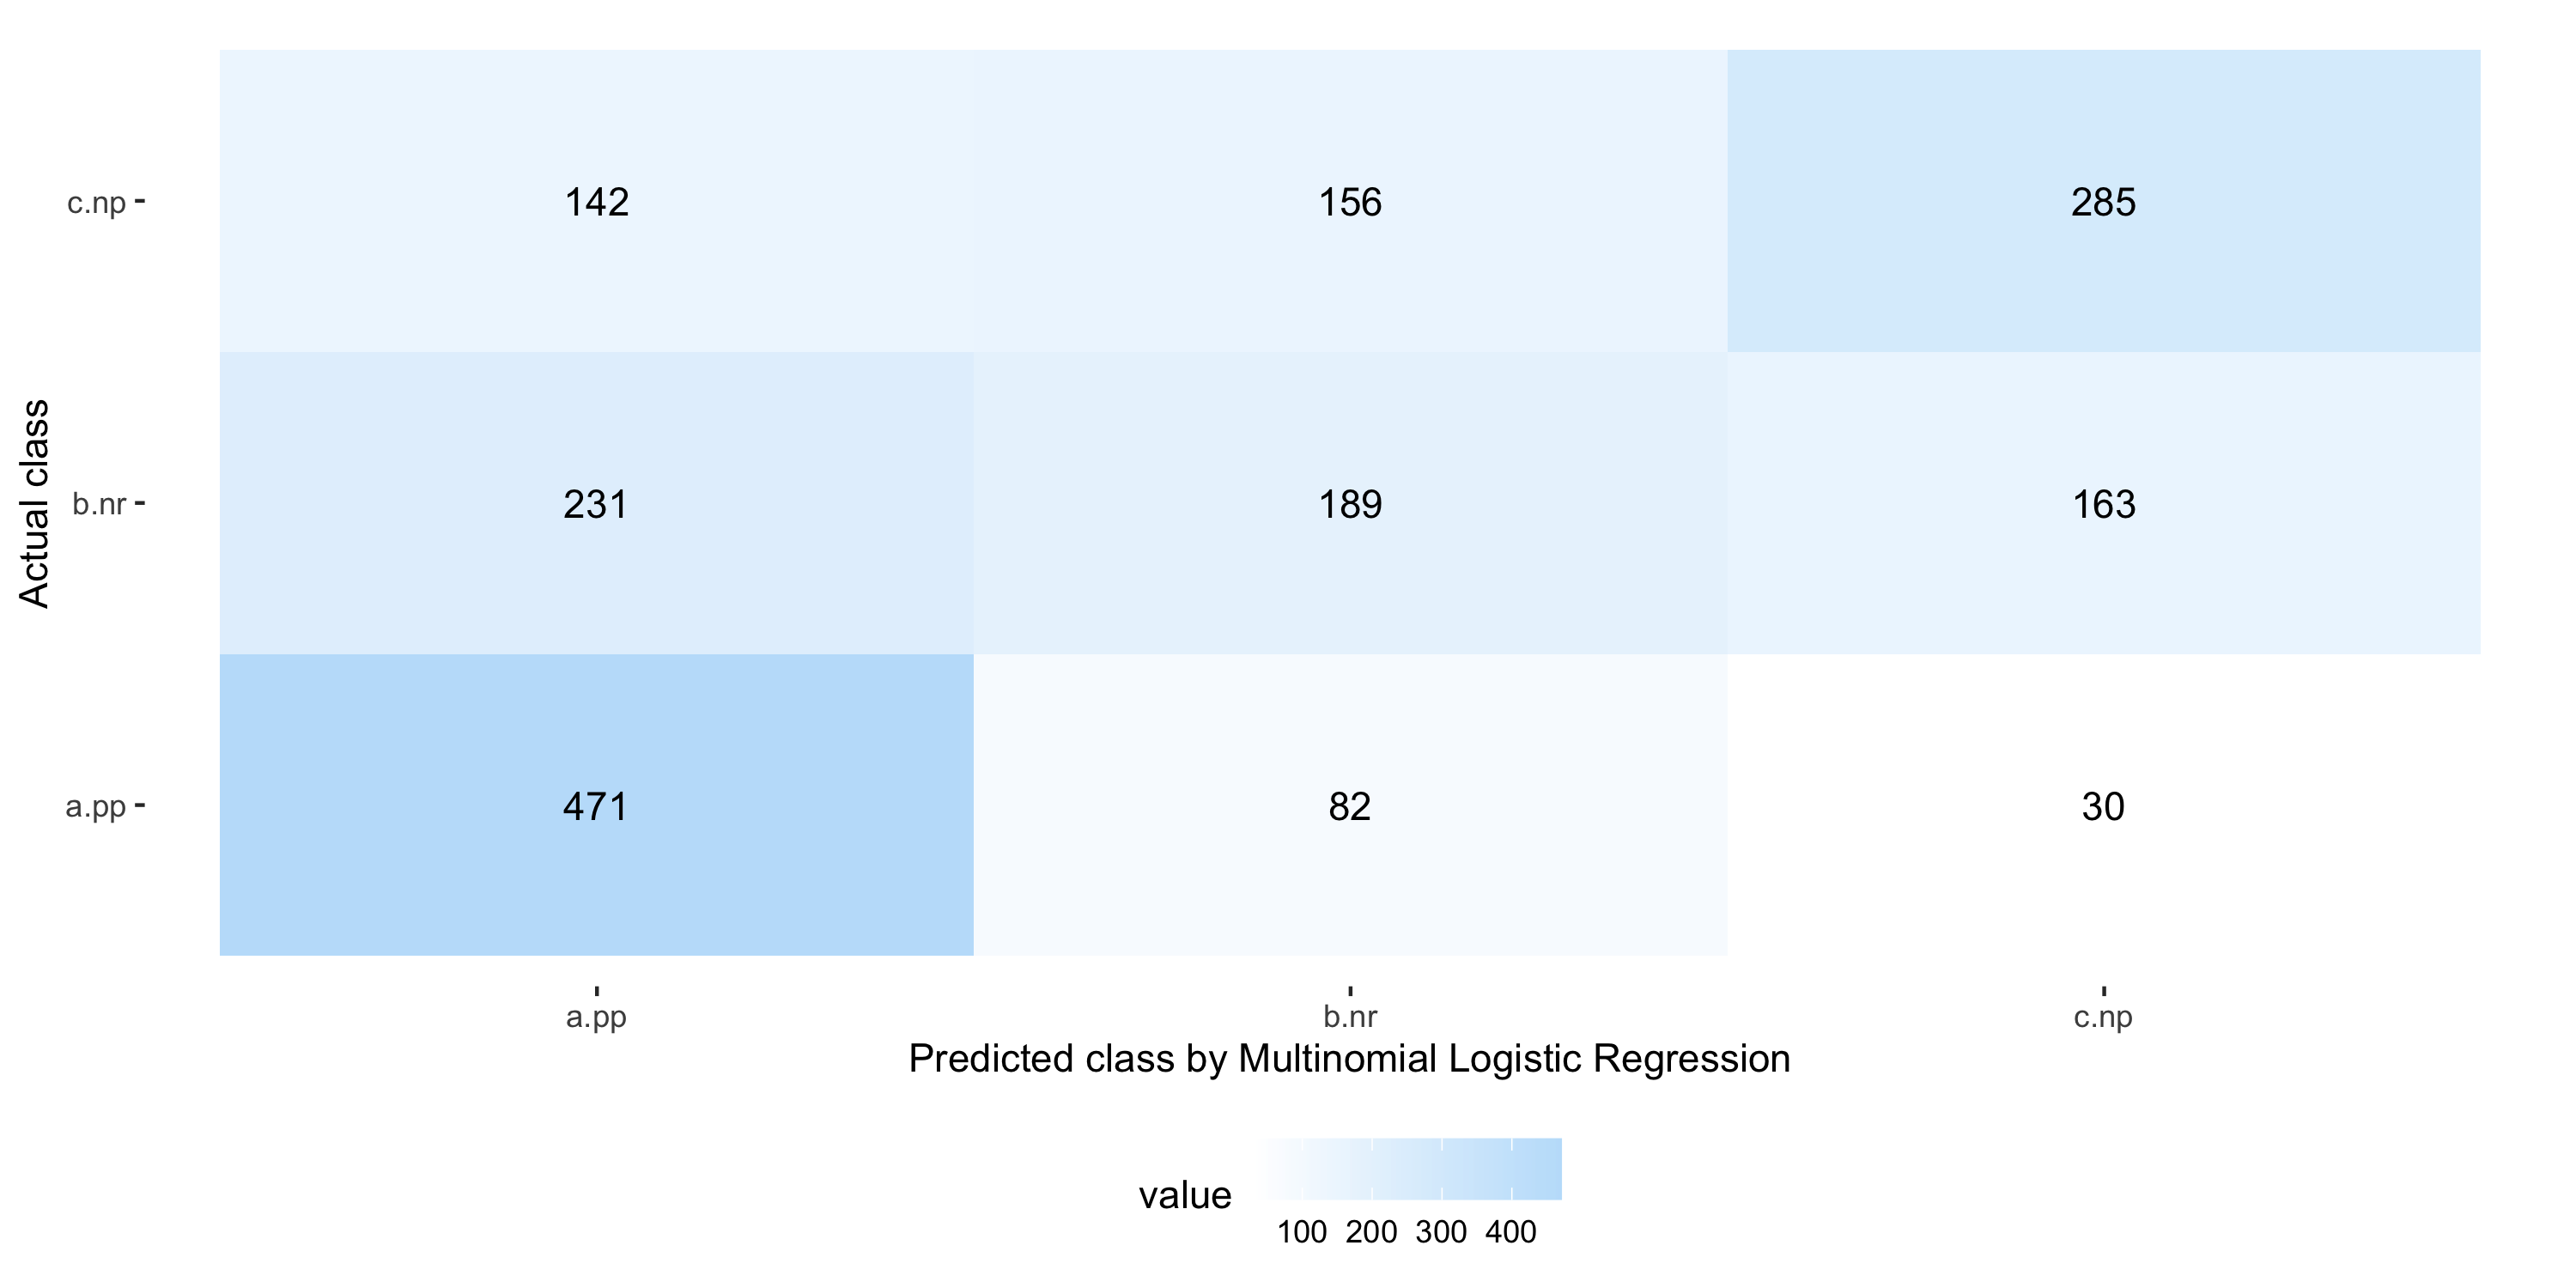
\includegraphics[width=0.4\textwidth]{figure/errorMultinomialLogisticRegression.png}}
\caption{Error Analysis\protect\footnotemark Of Multinomial Logistic Regression}
\label{errorMultinomialLogisticRegression}
\end{figure}
\footnotetext{The black line in the left figure is the average line of 10 accuracies in cross validation, and the overall accuracy in the right figure is from the best model picked from cross validation. All following similar figure are the same.}

\subsection{Linear Discriminative Analysis (LDA)}
After modeling LDA, we depicted and error analysis plot as Fig.\ref{errorLinearDiscriminativeAnalysis.pdf}. From error analysis plot we can see that the picked model's error rate is 0.516 which is almost the same as multinomial logistic regression. The prediction is almost no improvement, which means that both multinomial logistic regression and LDA can't greatly classify the data. 

As we all know, these two way generates a linear boundary of classification, however, when the real boundary is non-linear these 2 ways can't produce a great result. So we next try some non-linear boundary models.

\begin{figure}[htbp]
\centerline{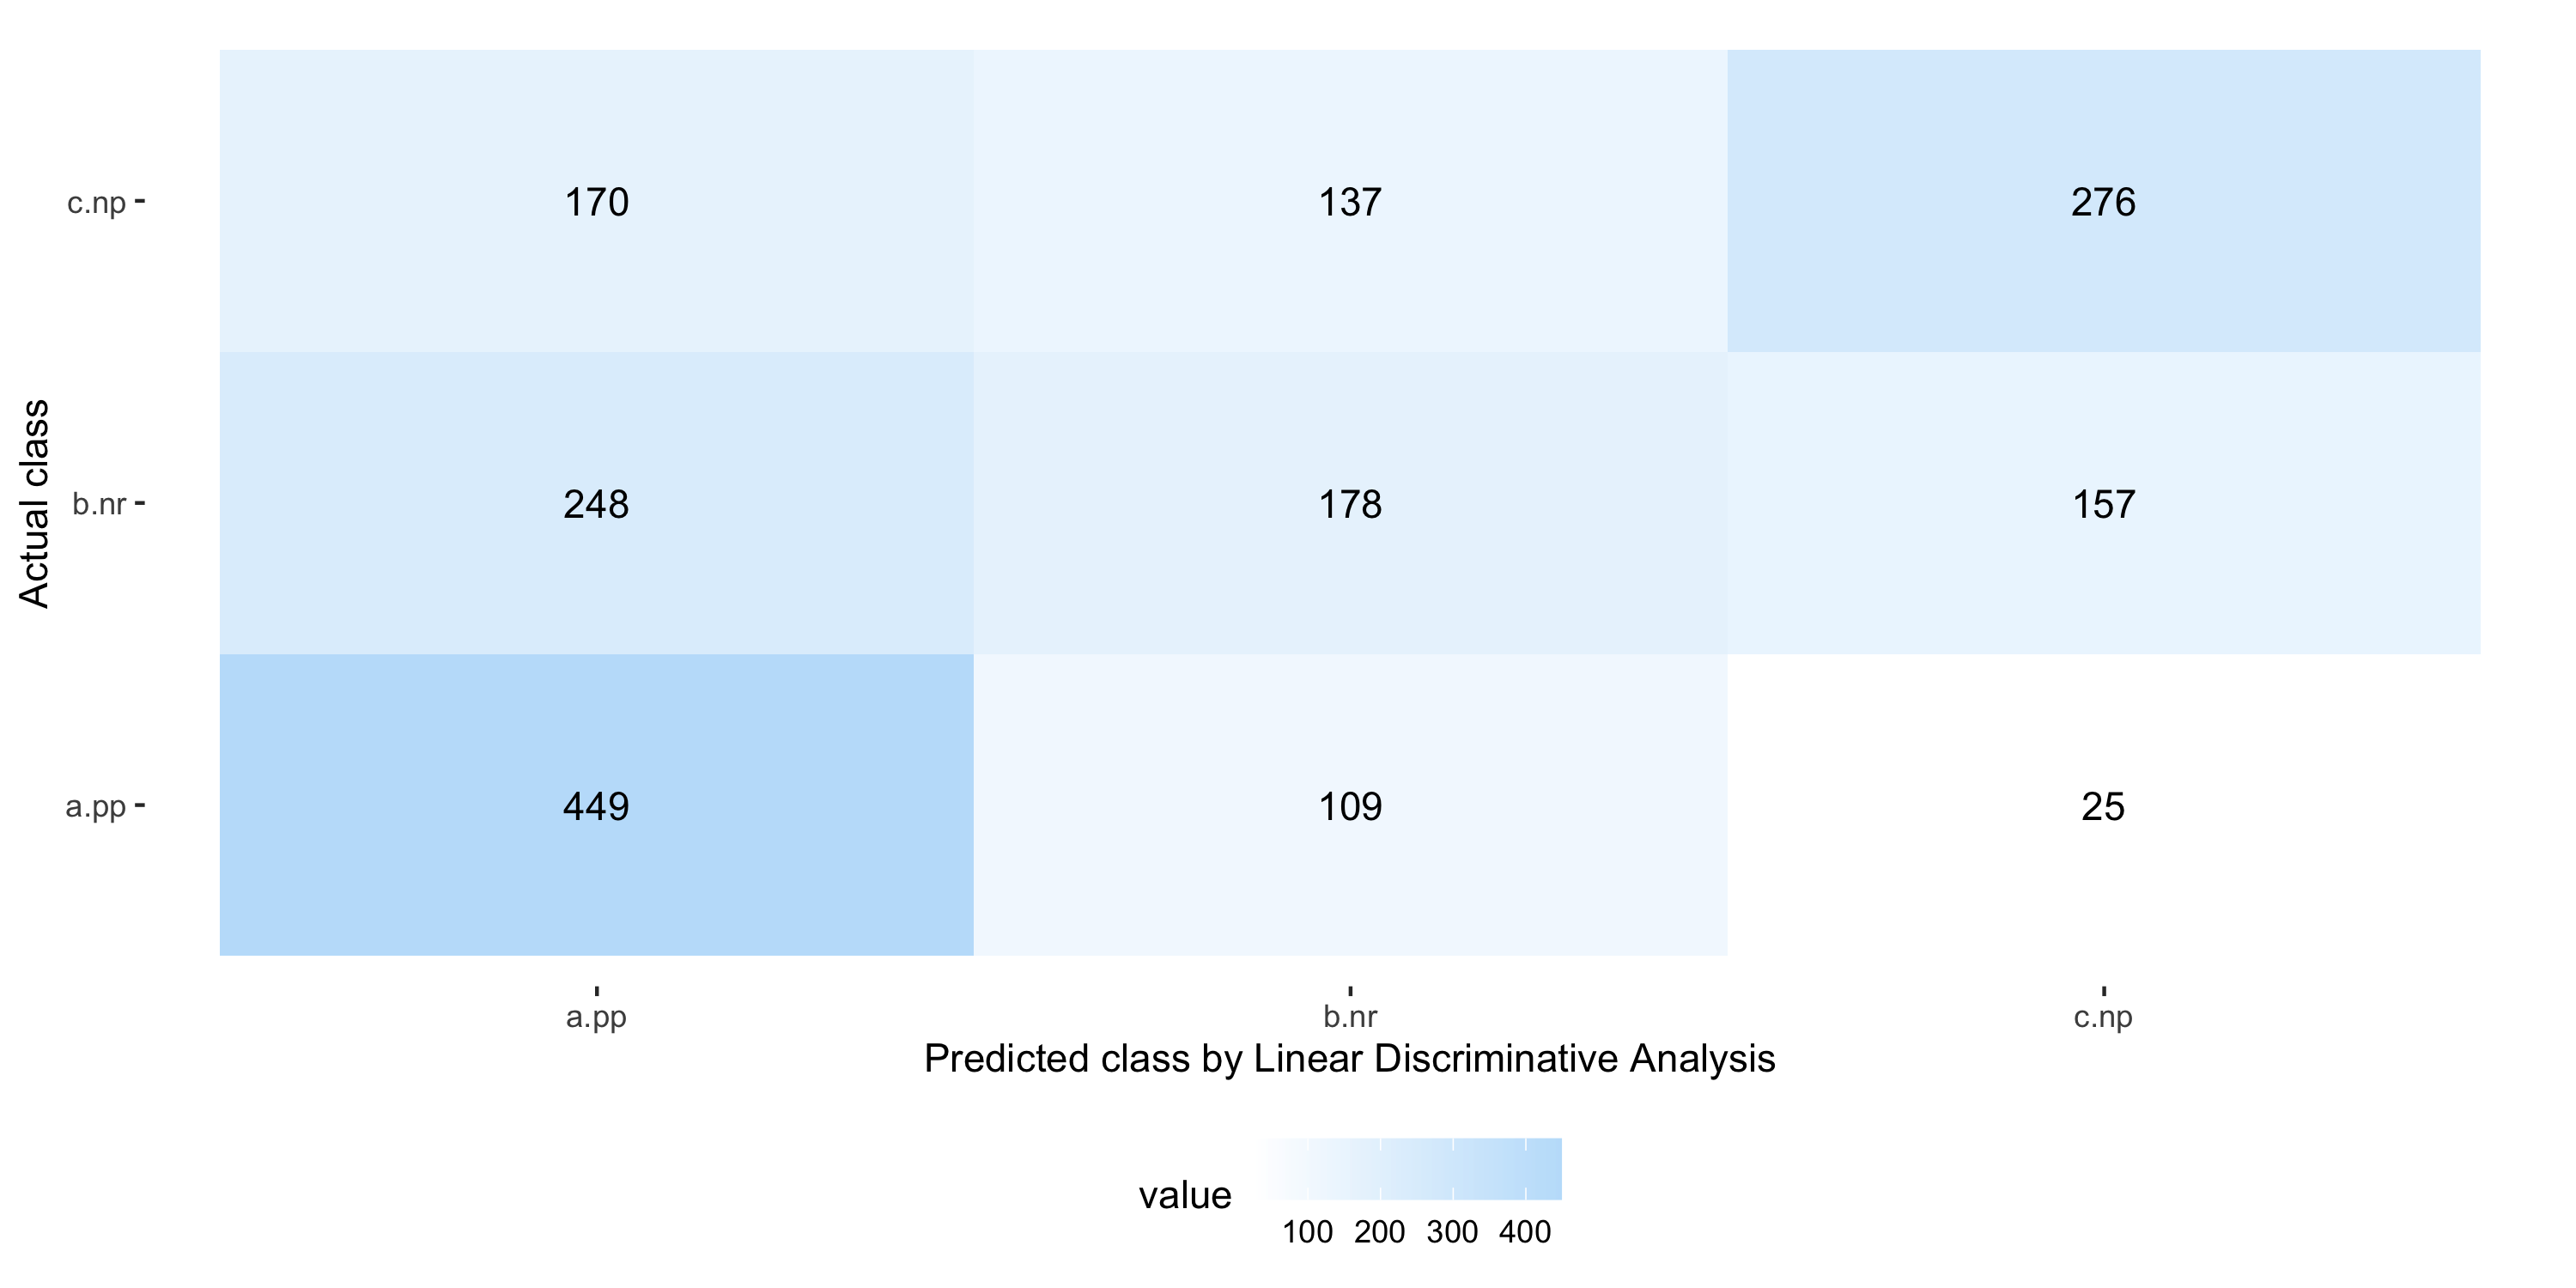
\includegraphics[width=0.4\textwidth]{figure/errorLinearDiscriminativeAnalysis.png}}
\caption{Error Analysis Of Linear Discriminative Analysis}
\label{errorLinearDiscriminativeAnalysis.pdf}
\end{figure}


\subsection{Quadratic Discriminative Analysis (QDA)}
In order to model a non-linear boundary, naturally, QDA comes to our mind. Since QDA assumes a quadratic decision boundary, it can accurately model a wider range of problems than the linear methods. 

We train the data with QDA model, and depicted error analysis plot as Fig.\ref{errorQuadraticDiscriminativeAnalysis.pdf}. From error analysis plot we can see that the picked model's error rate is 0.516. The overall prediction is the same as LDA which means that QDA is no better than previous ways. 


\begin{figure}[htbp]
\centerline{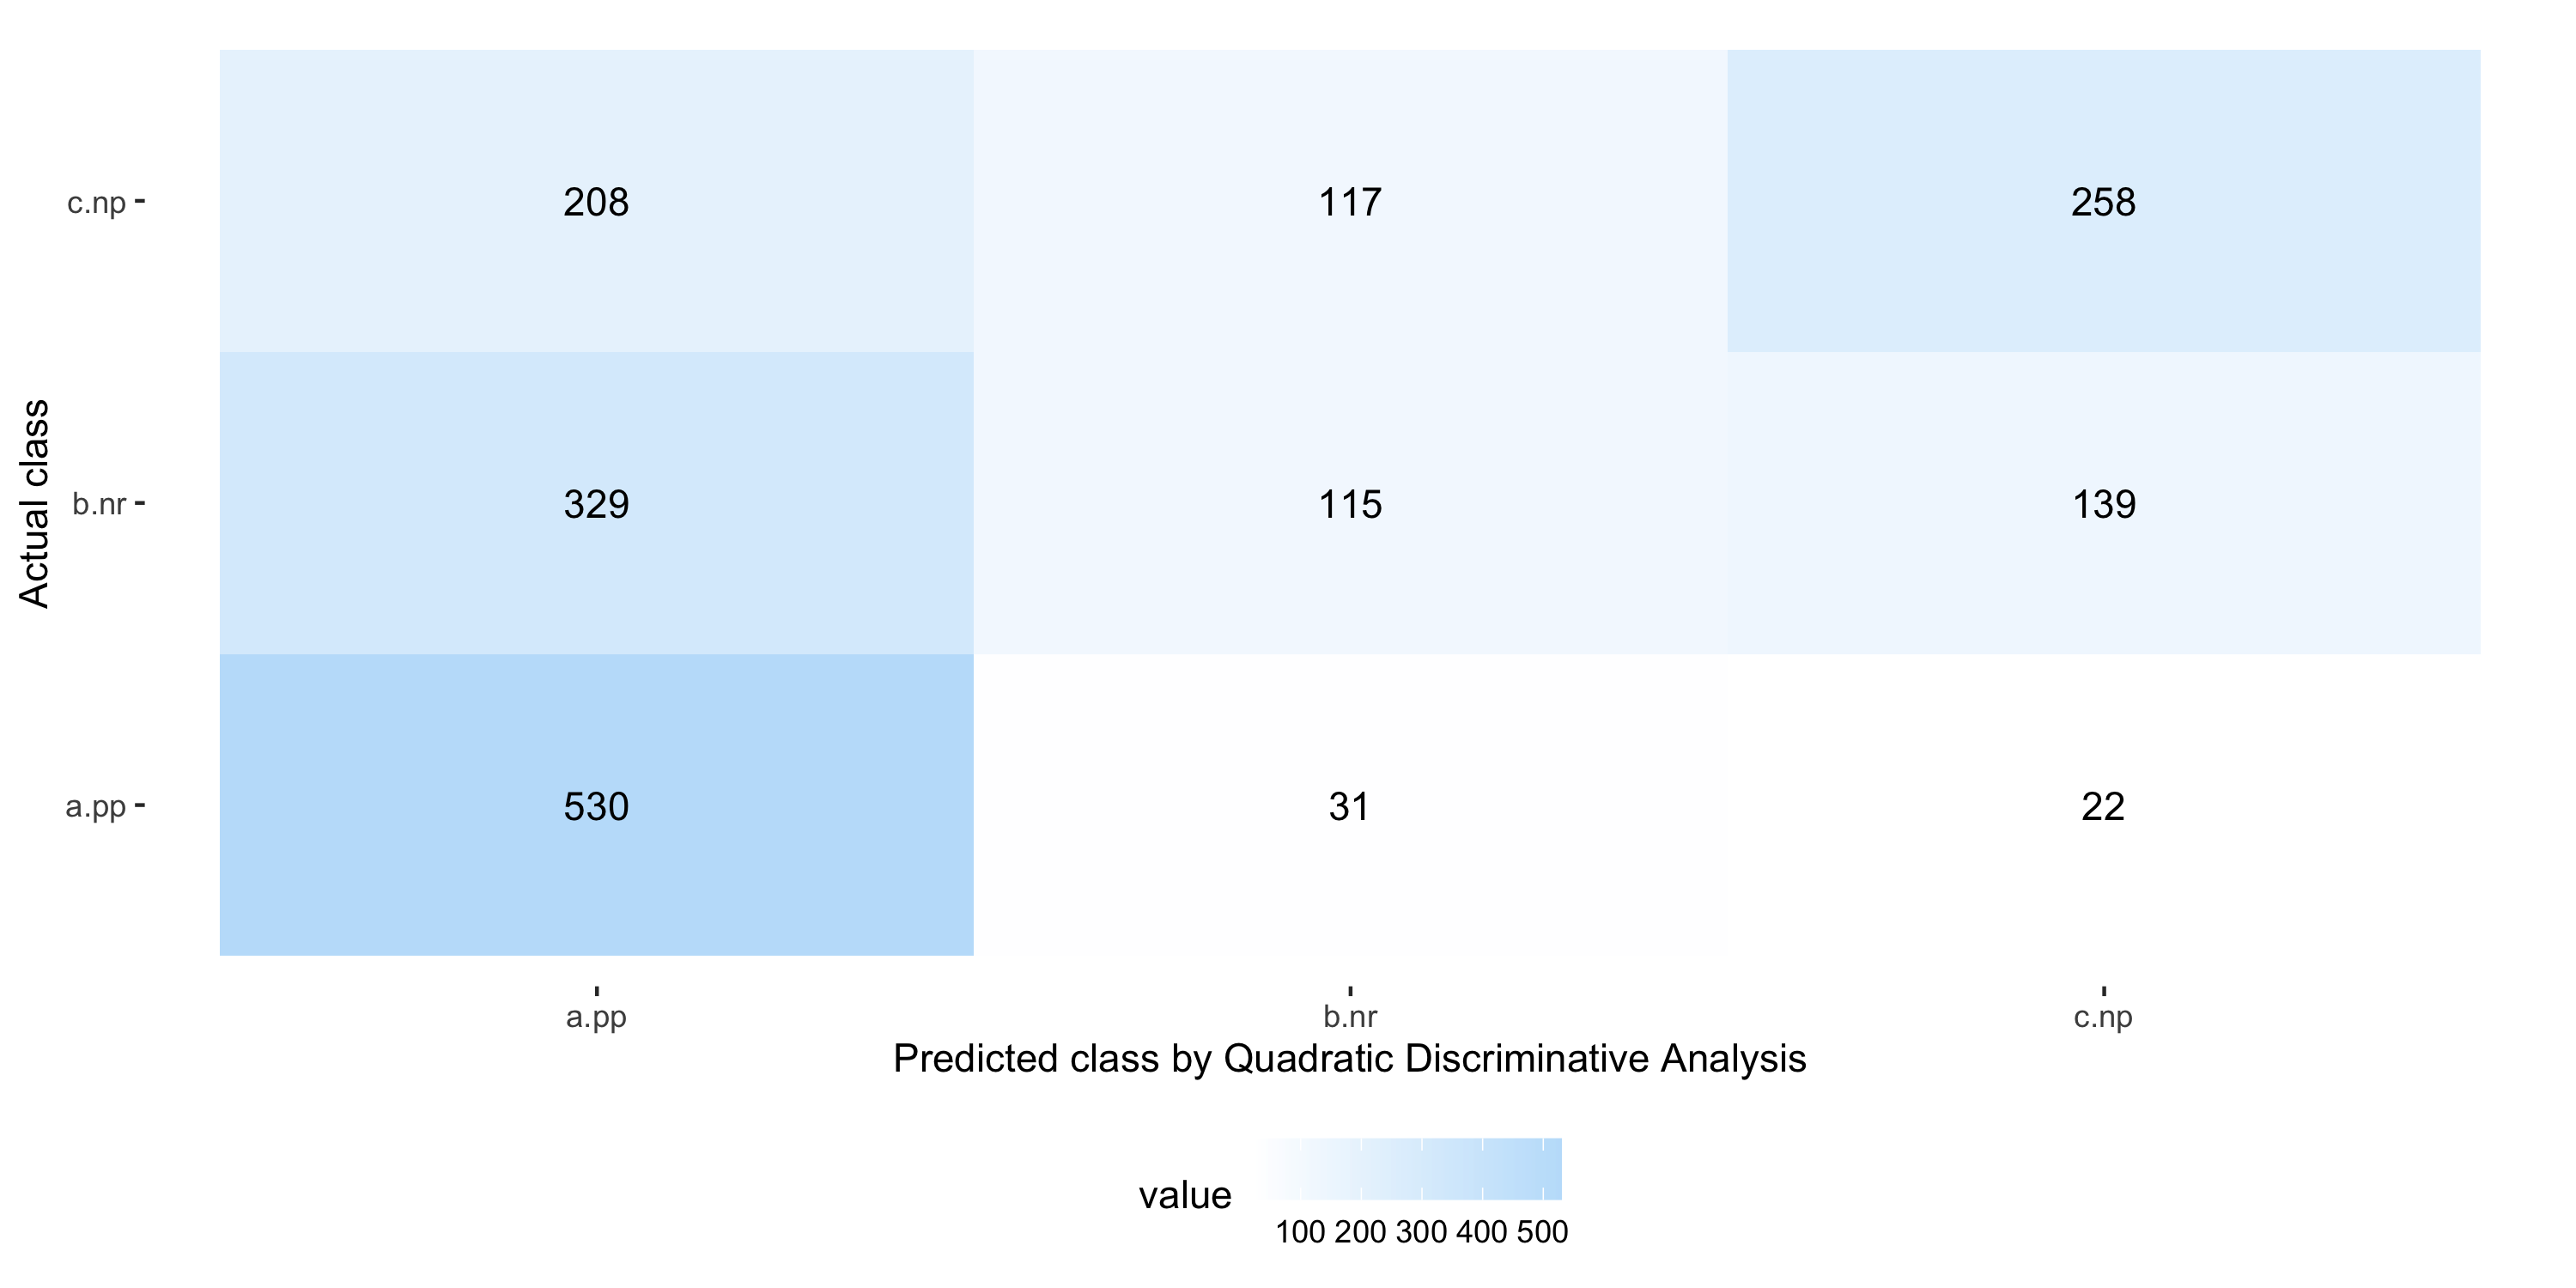
\includegraphics[width=0.4\textwidth]{figure/errorQuadraticDiscriminativeAnalysis.png}}
\caption{Error Analysis Of Quadratic Discriminative Analysis}
\label{errorQuadraticDiscriminativeAnalysis.pdf}
\end{figure}



\subsection{Decision Tree}
Besides, we train the data with Decision Tree model. Then we depict error analysis plot as Fig.\ref{errorDicisionTree.pdf}. From error analysis plot we can see that the picked model's error rate is 0.509 and it only predicted popular class greatly. Obviously, Decision Tree have no significant improvement than previous ways. 


\begin{figure}[htbp]
\centerline{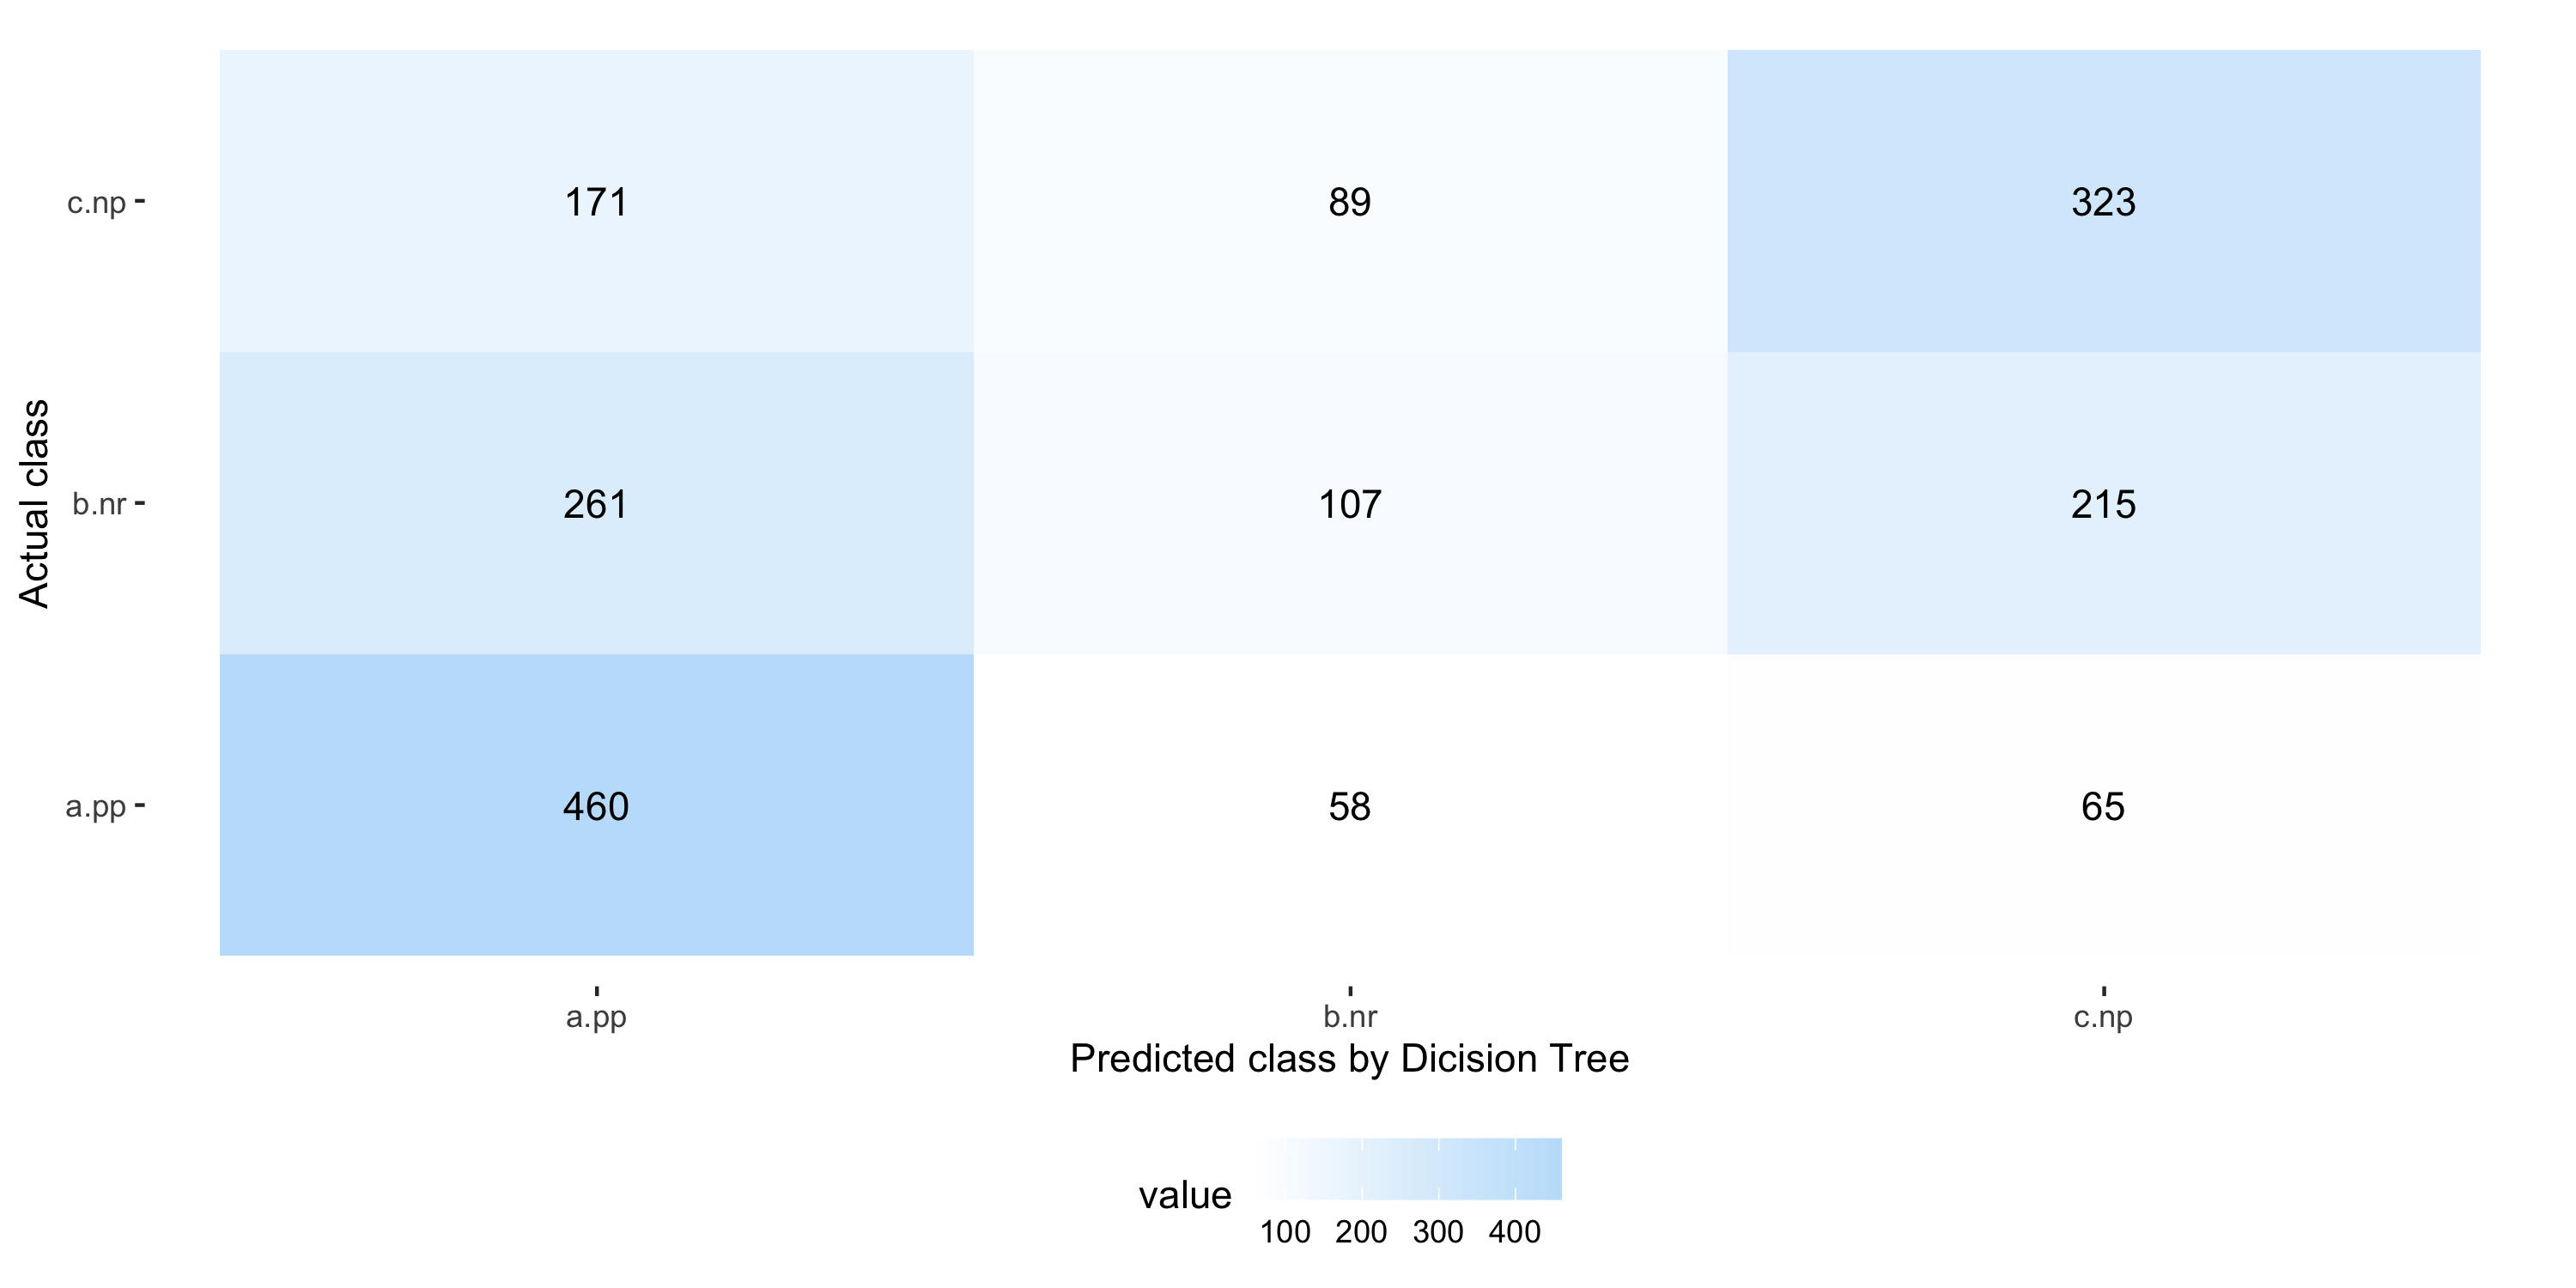
\includegraphics[width=0.4\textwidth]{figure/errorDicisionTree.png}}
\caption{Error Analysis Of Decision Tree Analysis}
\label{errorDicisionTree.pdf}
\end{figure}


% \subsection{Random Forest}
% We also tried to train the data with Random Forest model. Then we depict error analysis plot as Fig.\ref{errorRandomForest.pdf}. From error analysis plot we can see that the picked model's error rate is 0.509 and it only predicted normal class. Obviously, Decision Tree have no improvement than previous ways. 


% \begin{figure}[htbp]
% \centerline{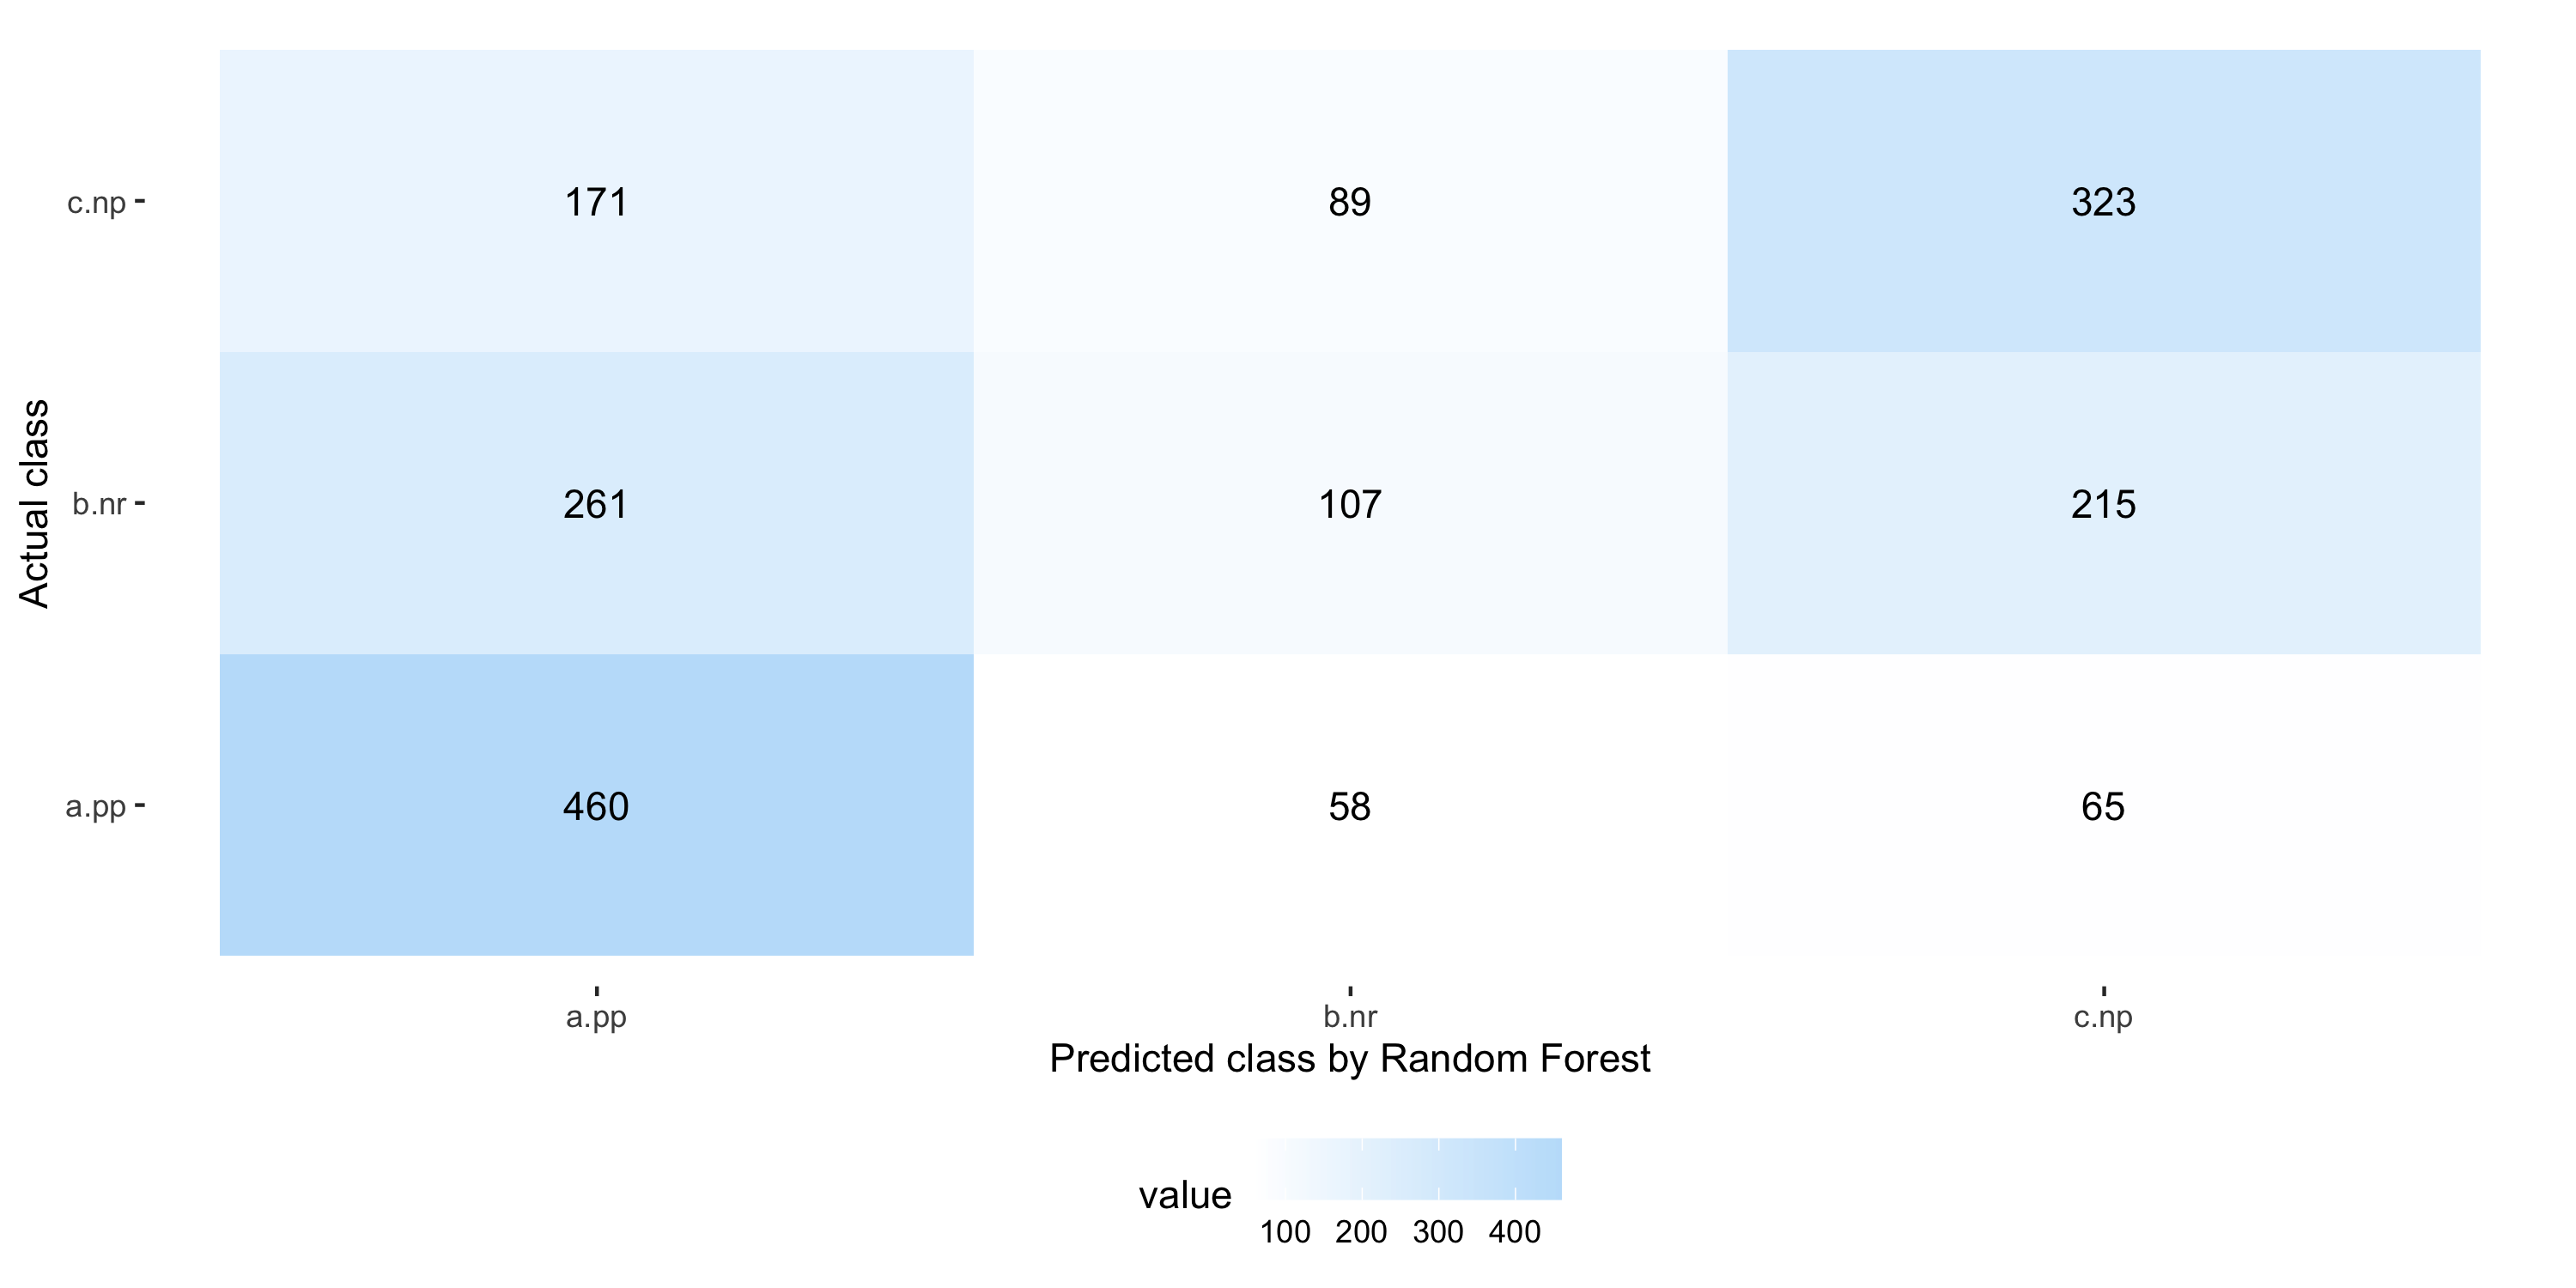
\includegraphics[width=0.4\textwidth]{figure/errorRandomForest.png}}
% \caption{Error Analysis Of Random Forest Analysis}
% \label{errorRandomForest.pdf}
% \end{figure}

\subsection{K-Nearest Neighbors (KNN)}
What if we use an even more flexible method than QDA? Will the result be better? Hence, KNN is introduced as our last classification method. We train the data with KNN model, get the best $k=2$ by cross validation. Then we depict error analysis plot as Fig.\ref{errorK-NearestNeighbors}. From error analysis plot we can see that the picked model's error is 0.391, and error rate on popular songs is 0.3953. The error rate has been decreased by 10\% than prior methods, however, the accuracy is still very low.

\begin{figure}[htbp]
\centerline{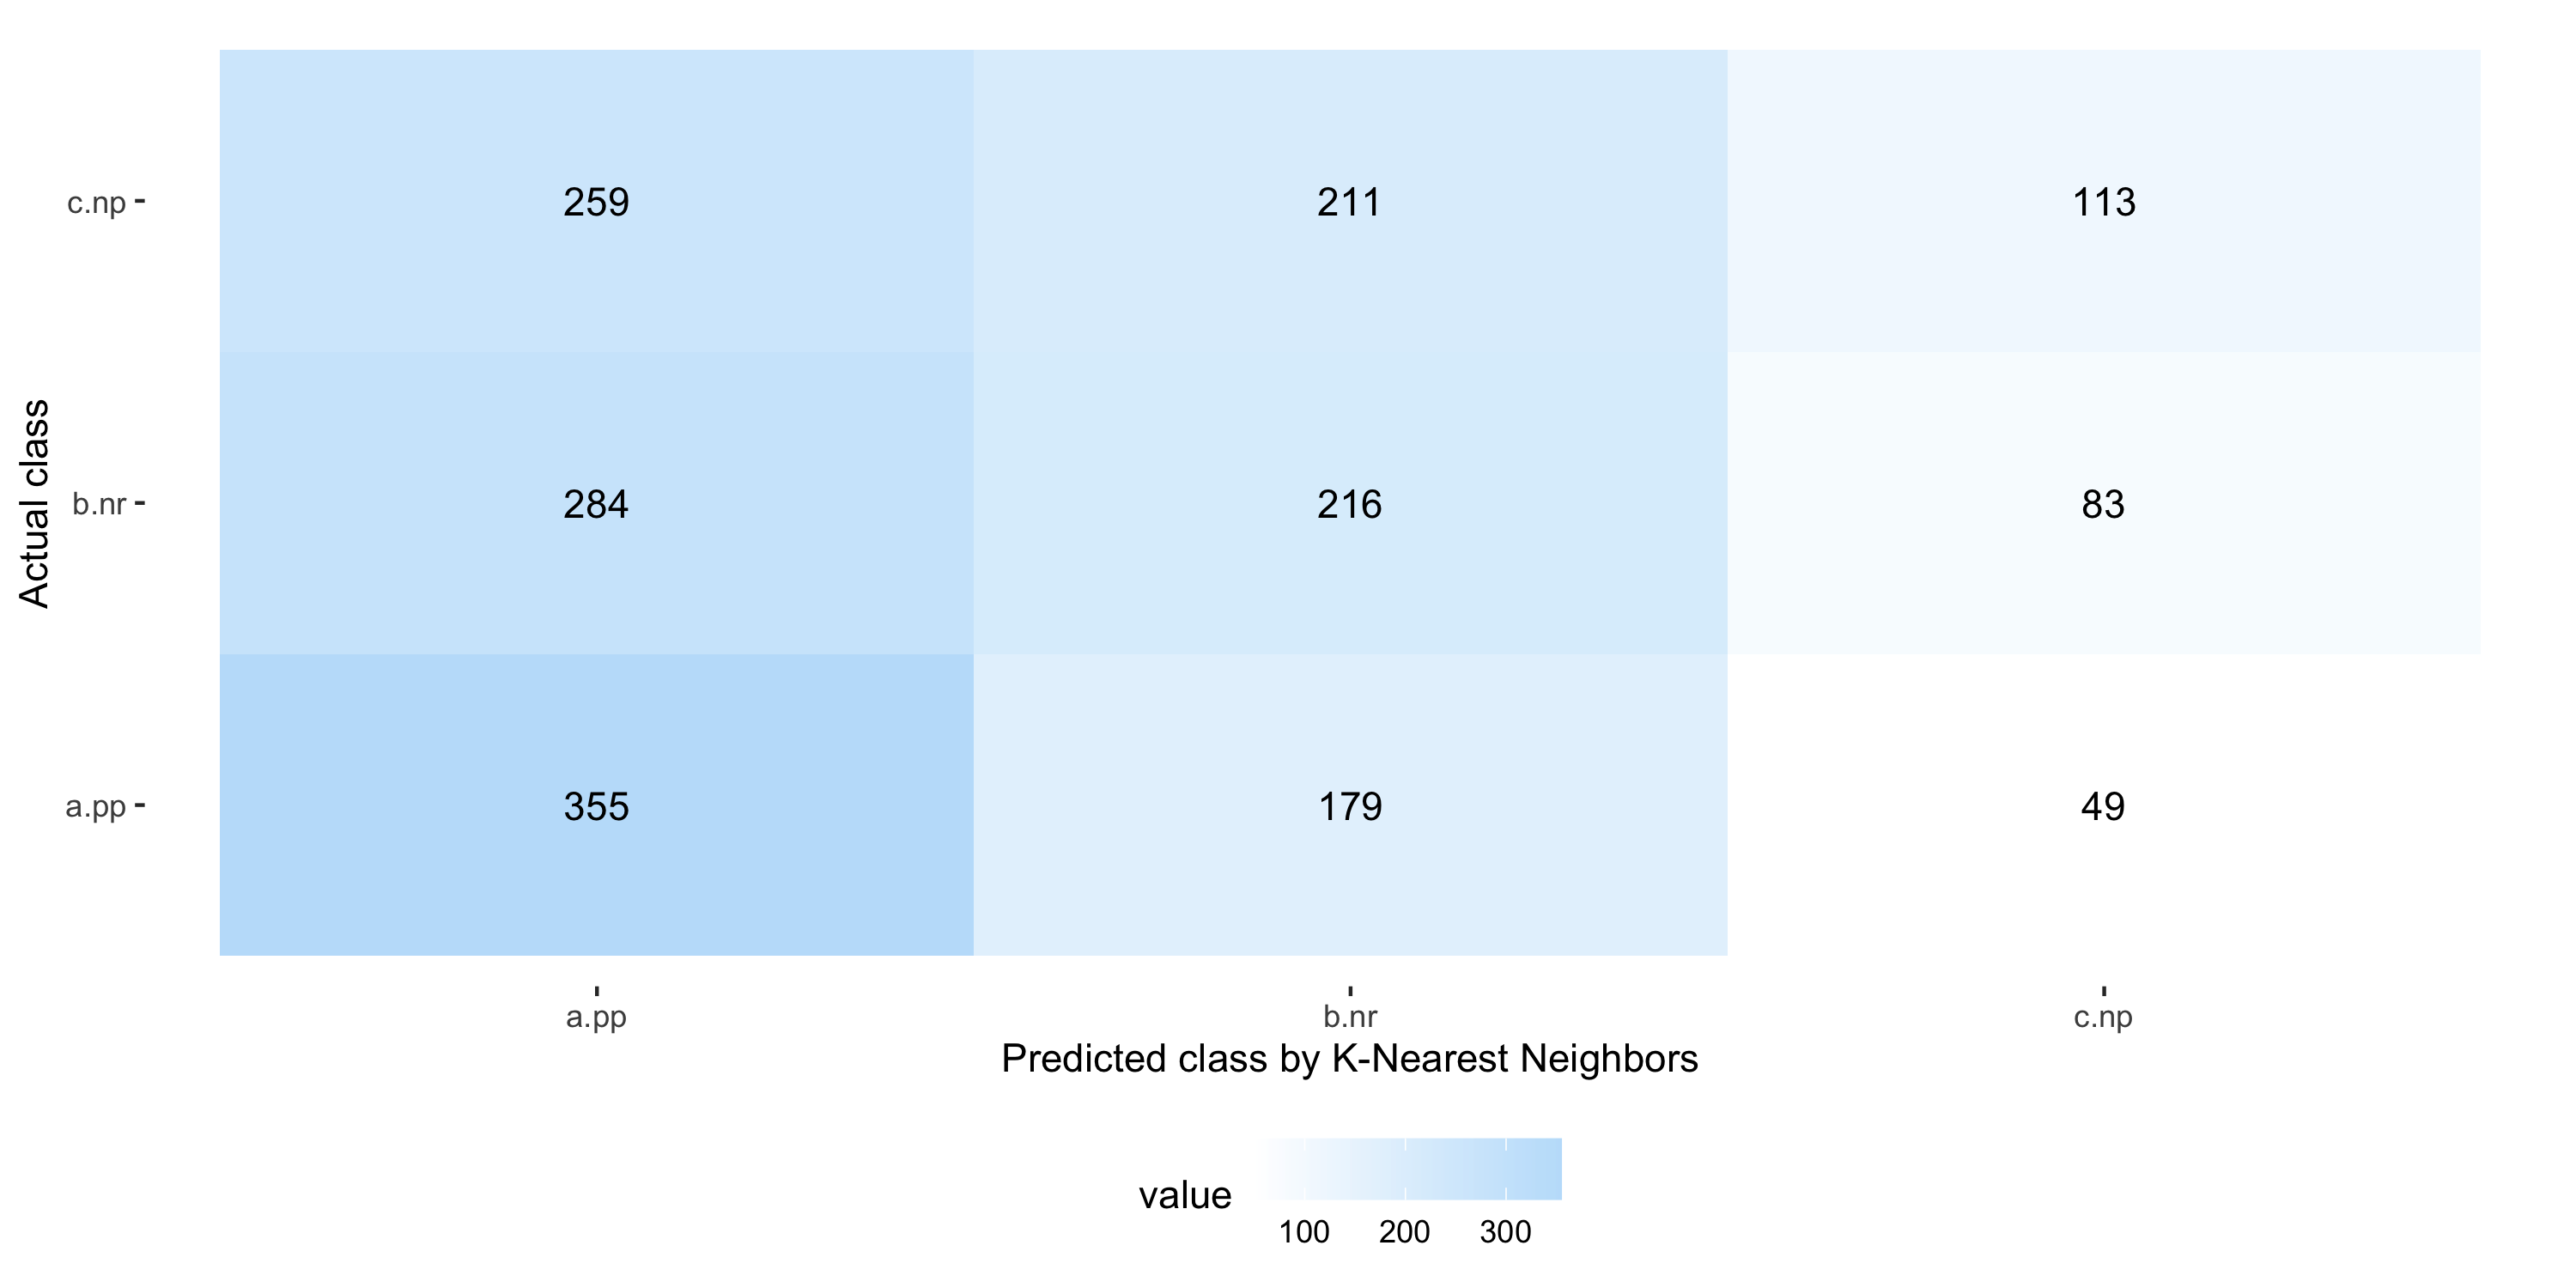
\includegraphics[width=0.4\textwidth]{figure/errorK-NearestNeighbors.png}}
\caption{Error Analysis Of 2-Nearest Neighbors Analysis}
\label{errorK-NearestNeighbors}
\end{figure}



\section{Conclusion}
Going into this endeavour, we were uncertain if it is even possible to predict, better than random, if a song will be popular or not. After testing our model on new songs pulling from Spotify, we observe that it is significantly simpler to correctly predict a bad song rather than a hit. It may have been easier to predict non hit songs because our data was skewed, with limited hit songs. Besides, We didn't consider lyrics,  to predict a song’s popularity.

From the result, we can see that all regression model are not so good. The error bar range in Fig. \ref{Total Number of Coefficient and RMSE in Ridge}, Fig. \ref{Total Number of Coefficient and RMSE in Lasso} and Fig. \ref{Total Number of Coefficient and RMSE in Elastic-net} is large. 

\section{Futrue works}
Moving forward, we would like to explore how additional features such as lyrics, artist popularity, artist location or release date can influence a song’s popularity. In addition, we may consider using the full dataset to see if we can improve our models. Another alternative is to use Spotify API to collect our own data.

% \section*{Acknowledgment}

% I would like to express my special thanks of gratitude to my teacher who gave me the golden opportunity to do this wonderful project on the topic of this, which also helped me in doing a lot of Research and I came to know about so many new things I am really thankful to him.


\bibliography{IEEEabrv,references}
\bibliographystyle{IEEEtran}

\vspace{12pt}
%\color{red}
%IEEE conference templates contain guidance text for composing and formatting conference papers. Please ensure that all template text is removed from your conference paper prior to submission to the conference. Failure to remove the template text from your paper may result in your paper not being published.

\clearpage
\newpage


\appendices
\section{R Source Code}
\label{FirstAppendix}
\lstinputlisting[language=java]{../Code/Final project.R}
\end{document}
